\documentclass[10pt,english,aspectratio=169]{beamer}
% Use notes or hide notes or show only notes or handout


\usetheme{default}

\usepackage{xstring}
\usepackage{pgfpages}
%\makeatletter
%\IfSubStr{\@classoptionslist}{handout}
%  {\pgfpagesuselayout{2 on 1}[letterpaper,border shrink=5mm]}
%  {}
%\makeatother

\usepackage{amsmath,amssymb,amsthm}
\usepackage{stmaryrd}
\usepackage{enumerate}
\usepackage{stfloats}
\usepackage{bbm}
\usepackage{pdfpages}
\usepackage{framed}

\usepackage[most]{tcolorbox}
\tcbset{highlight math style={enhanced,
  colframe=white,colback=yellow!15,arc=8pt,boxrule=1pt,
  }}
  
\usepackage{tikz,pgf,pgfplots}
\usepackage{algorithm,algorithmic}
\usepgflibrary{shapes}
\usetikzlibrary{%
  arrows,%
  arrows.meta,
  shapes.misc,% wg. rounded rectangle
  shapes.arrows,%
  shapes,%
  calc,%
  chains,%
  matrix,%
  positioning,% wg. " of "
  scopes,%
  decorations.pathmorphing,% /pgf/decoration/random steps | erste Graphik
  shadows,%
  backgrounds,%
  fit,%
  petri,%
  quotes
}

\setbeamersize{text margin left=10mm,text margin right=35mm}

\pgfplotsset{compat=1.12}

%\usetheme{Frankfurt}
%\usecolortheme{ldpc}
\useinnertheme{rounded}
\usecolortheme{whale}
\usecolortheme{orchid}

\newcommand{\ul}[1]{\underline{#1}}
\renewcommand{\Pr}{\mathbb{P}}

%% Setup slides and notes
\makeatletter
\IfSubStr{\@classoptionslist}{notes} { \IfSubStr{\@classoptionslist}{hide} {}{\IfSubStr{\@classoptionslist}{only} {}{\setbeameroption{show notes on second screen=right}}} }{}
\makeatother
%\setbeamertemplate{note page}{\pagecolor{yellow!5}\vfill\insertnote\vfill}

\newcommand{\getpdfpages}[2]{\begingroup
  \setbeamercolor{background canvas}{bg=}
  \addtocounter{framenumber}{1}
  \includepdf[pages={#1},%
  pagecommand={%
    \expandafter\def\expandafter\insertshorttitle\expandafter{%
      \insertshorttitle\hfill\insertframenumber\,/\,\inserttotalframenumber}}%
  ]{#2}
  \endgroup}

\newcommand{\backupbegin}{
   \newcounter{finalframe}
   \setcounter{finalframe}{\value{framenumber}}
}
\newcommand{\backupend}{
   \setcounter{framenumber}{\value{finalframe}}
}

 \setbeamercolor{bibliography entry author}{fg=black}
 \setbeamercolor{bibliography entry title}{fg=black}
 \setbeamercolor{bibliography entry location}{fg=black}
 \setbeamercolor{bibliography entry note}{fg=black}
 
 \setbeamerfont{bibliography item}{size=\footnotesize}
 \setbeamerfont{bibliography entry author}{size=\footnotesize}
 \setbeamerfont{bibliography entry title}{size=\footnotesize}
 \setbeamerfont{bibliography entry location}{size=\footnotesize}
 \setbeamerfont{bibliography entry note}{size=\footnotesize}
 \setbeamertemplate{bibliography item}{\insertbiblabel}
 
\newlength\tikzwidth
\newlength\tikzheight


\newcommand{\mc}[1]{\mathcal{#1}}
\newcommand{\mbb}[1]{\mathbb{#1}}
\newcommand{\expt}{\mbb{E}}
\newcommand{\dd}{\mathrm{d}}

\def\checkmark{\tikz\fill[scale=0.4](0,.35) -- (.25,0) -- (1,.7) -- (.25,.15) -- cycle;}
\def\greencheck{{\color{green}\checkmark}}
\def\scalecheck{\resizebox{\widthof{\checkmark}*\ratio{\widthof{x}}{\widthof{\normalsize x}}}{!}{\checkmark}}
\def\xmark{\tikz [x=1.4ex,y=1.4ex,line width=.2ex, red] \draw (0,0) -- (1,1) (0,1) -- (1,0);}
\def\redx{{\color{red}\xmark}}

\renewcommand{\footnotesep}{-2pt}

\newif\ifslow
\slowtrue

\newcommand{\vecnot}[1]{#1}

\begin{document}

\ifslow

\title{ECE 586: Vector Space Methods \\ Lecture 4 Flip Video: Relations and Functions}
\author{Henry D. Pfister \\ Duke University}
\date{}
%\date{August 20th, 2020}
%\maketitle

\setbeamertemplate{navigation symbols}{}

\begin{frame}[plain]
	\titlepage
	
	\note{
		\vspace{8mm}
		\begin{enumerate}
			\setlength\itemsep{3mm}
			\color{red}
			\item Welcome to the fourth video lecture for ECE 586, Vector Space Methods. \\[2mm]
			Today, we'll discuss equivalence relations and functions.
		\end{enumerate}
	}
\end{frame}

\addtocounter{framenumber}{-1}
\setbeamertemplate{navigation symbols}{\textcolor{blue}{\footnotesize \insertframenumber ~/ \inserttotalframenumber}}


\begin{frame}{1.4: Cartesian Products and Abstract Relations}

\vspace{-2mm}

\begin{itemize}
\setlength\itemsep{3mm}

\item<1-> Sets of tuples and vectors \vspace{1mm}
\begin{itemize}
  \setlength\itemsep{1.5mm}
  %Build sets by grouping elements into vectors
  \item For sets $A,B$, the \textcolor{blue}{Cartesian product} $A\times B$ is the set of ordered pairs \[ A \times B \triangleq \{(a,b) \,|\, a\in A, b\in B\}\]
  \item For $n$-tuples from the same set, we write $A^n=A\times A \times \cdots \times A$
  \item Ex. For $A  = \{ a,b \}$ and $B  = \{ c,d \}$, we have
\begin{align*}
A\times B &= \{(a,c),(a,d),(b,c),(b,d) \} \\
A^2 = A \times A &= \{ (a,a),(a,b),(b,a),(b,b) \} \\
\!\!\!\!\!\!\!\!\!\!\!\!\!\!\!\!\!\!\! A^3 = \{ (a,a,a),(a,a,b),&(a,b,a),(a,b,b),(b,a,a),(b,a,b),(b,b,a),(b,b,b) \} \\
\end{align*}
\end{itemize}
\end{itemize}
\vspace{-7mm}

\begin{definition}<2->
A \textcolor{blue}{relation} $\sim$ between elements of $A$ is defined by the subset $R \subseteq A\times A$.  Specifically, we say the relation $x \sim y$ holds if and only if $(x,y)\in R$.
\end{definition}
\uncover<2->{Relations are the abstraction of operators like $\{\, = \, , \, \leq \, , \, \geq \, , \, < \, , \, > \, \}$}

\note{
	\vspace{8mm}
	\begin{enumerate}
		\setlength\itemsep{3mm}
		\color{red}
		\item Read.  
		\item Read. 
	\end{enumerate}
}


\end{frame}



\begin{frame}<1-5> \frametitle{1.4: Properties of Relations}

\begin{itemize}
\setlength\itemsep{5mm}
\item<1-> The relation $\sim$ on $A$ is said to be: \vspace{1mm}
\begin{itemize}
  \setlength\itemsep{1.5mm}
  \item \textcolor{blue}{Reflexive} if $x\sim x$ holds for all $x\in A$ $\;\;$ (i.e., $\forall x\in A, (x,x) \in R$)
  \item \textcolor{blue}{Symmetric} if $x\sim y$ then $y\sim x$ for all $x,y\in A$
  \item \textcolor{blue}{Transitive} if $x\sim y$ and $y\sim z$, then $x\sim z$ for all $x,y,z\in A$
\end{itemize}

\item<2-> It is an \textcolor{blue}{equivalence relation} if it is reflexive, symmetric, and transitive \vspace{1mm}

\begin{itemize}
  \setlength\itemsep{1.5mm}
  %\item Abstract generalization of equality
  \item Ex. let $A$ be a set of people and $P(x,y)$ be the statement: \\ \textcolor{blue}{``$x$ has the same birthday (month and day) as $y$''}
  \item Define \textcolor{blue}{relation $\sim$} such that \textcolor{blue}{$x\sim y$} holds iff $P(x,y)$ is true.  Then, \vspace{-1mm}
  \[ R = \{ (x,y)\in A\times A \,|\, P(x,y) \} \vspace*{-1mm} \]
  \item<3-> Partitions $A$ into disjoint \textcolor{blue}{equivalence classes}: $[a] \triangleq \left\{x\in A | x \sim a\right\}$
  \item<4-> Ex. $\sim$ has an equivalence class for each possible day in a year
  \item<5-> Set of equivalence classes called the \textcolor{blue}{quotient set}: $A / \!\sim \;\triangleq \{ \, [a] \, | \, a\in A \}\!\!\!\!\!$

\end{itemize}
\end{itemize}

\note{
	\vspace{8mm}
	\begin{enumerate}[<alert@+>]
		\footnotesize
		\setlength\itemsep{3mm}
		\item Read.  
		\item Read.  Check conditions.
		\item Read.  Here, the brackets around $a$ (i.e., $[a]$) represents all elements that are equivalent to $a$.  Notice that every element must be in some equivalence class.  Also, no element can be in two different equivalence classes due to transitivity.
		\item Read.
		\item Read.  The quotient set can be seen as the collection of subsets that partition $A$.
	\end{enumerate}
}

\end{frame}

\begin{frame}{1.5: Functions}

\vspace{3mm}

\begin{definition}
A \textcolor{blue}{function} $f \colon X \rightarrow Y$ from $X$ to $Y$ is defined by a subset $F \subset X \times Y$ such that $A_x = \{ y\in Y | (x,y)\in F \}$ has exactly one element for each $x\in X$.
The \textcolor{blue}{value} of $f$ at $x\in X$, \textcolor{blue}{denoted $f(x)$}, is unique element in $A_x$.
\end{definition}

\begin{itemize}
\setlength\itemsep{3mm}
\item<2-> Unpacking the definition \vspace{1mm}
\begin{itemize} 
  \setlength\itemsep{1.5mm}
  \item<2-> Function $f \colon X\rightarrow Y$ assigns one value $f(x)\in Y$ to each $x\in X$
  \item<3-> Notation \textcolor{blue}{$f \colon X \rightarrow Y$} emphasizes the \textcolor{blue}{domain} $X$ and the \textcolor{blue}{codomain} $Y$
  \item<4-> \textcolor{blue}{Range} of $f$ is subset of $Y$ achieved by $f$, $\{y \in Y \,|\, \exists x\in X, y=f(x) \}$
  \item<5-> Since the term codomain is uncommon, people sometimes use the term range instead of codomain either intentionally or unintentionally
\end{itemize}

\item<6-> In basic math, functions are often described by graphs and formulas \vspace{1mm}
\begin{itemize} 
  \setlength\itemsep{1.5mm}
  \item<6-> This leads students to picture only ``nice'' functions
  \item<7-> Ex. Cauchy published \textcolor{blue}{incorrect proof of the false assertion}: ``a sequence of continuous functions converging everywhere has a continuous limit''
  %\item Teachers now warn: \textcolor{blue}{the world is filled with ``not so nice'' functions}
\end{itemize}

\end{itemize}
\end{frame}  

\begin{frame}{1.5: Properties of Functions}

\begin{itemize}
\setlength\itemsep{3mm}
\item<1-> Equality \vspace{1mm}
\begin{itemize}
  \setlength\itemsep{1.5mm}
  \item Two functions are \textcolor{blue}{equal} if they have the same domain, codomain, and value for all elements of the domain
\end{itemize}

\item<2-> A function $f \colon X \to Y$ is called: \vspace{1mm}
\begin{itemize}
  \setlength\itemsep{1.5mm}
  \item \textcolor{blue}{one-to-one} or \textcolor{blue}{injective} if, $\forall x,x'\in X$, if $f(x)=f(x')$ then $x=x'$
  \item \textcolor{blue}{onto} or \textcolor{blue}{surjective} if its range $\{ f(x) | x\in X\}$ equals $Y$
  \item \textcolor{blue}{one-to-one correspondence} or \textcolor{blue}{bijective} if both one-to-one and onto
\end{itemize}

\item<3-> Inversion \vspace{1mm}
\begin{itemize}
  \setlength\itemsep{1.5mm}
  \item A bijective function has a unique \textcolor{blue}{inverse function} $f^{-1} \colon Y\rightarrow X$ satisfying: $\forall x\in X, f^{-1}(f(x)) = x$ and $\forall y\in Y, f(f^{-1}(y)) = y$
  \item Any one-to-one function $f \colon X\rightarrow Y$ defines a bijective function $g \colon X \rightarrow R$ where $R$ is the range of $f$ and $g(x)=f(x)$ for all $x\in X$

\end{itemize}

\end{itemize}
\end{frame}    


\begin{frame}<1-3> \frametitle{1.5: Applying Functions to Sets (1)}

\vspace{1mm}
\begin{definition}<1->
For $f \colon X\rightarrow Y$ and subset $A\subseteq X$, the \textcolor{blue}{image} of $A$ under $f$ is \vspace{-2mm}
\[ f(A) \triangleq \{ y\in Y | \exists x\in A \textrm{ s.t. } f(x)=y\} = \{f(x) | x\in A\}. \]
\end{definition}

\begin{center}
\uncover<2->{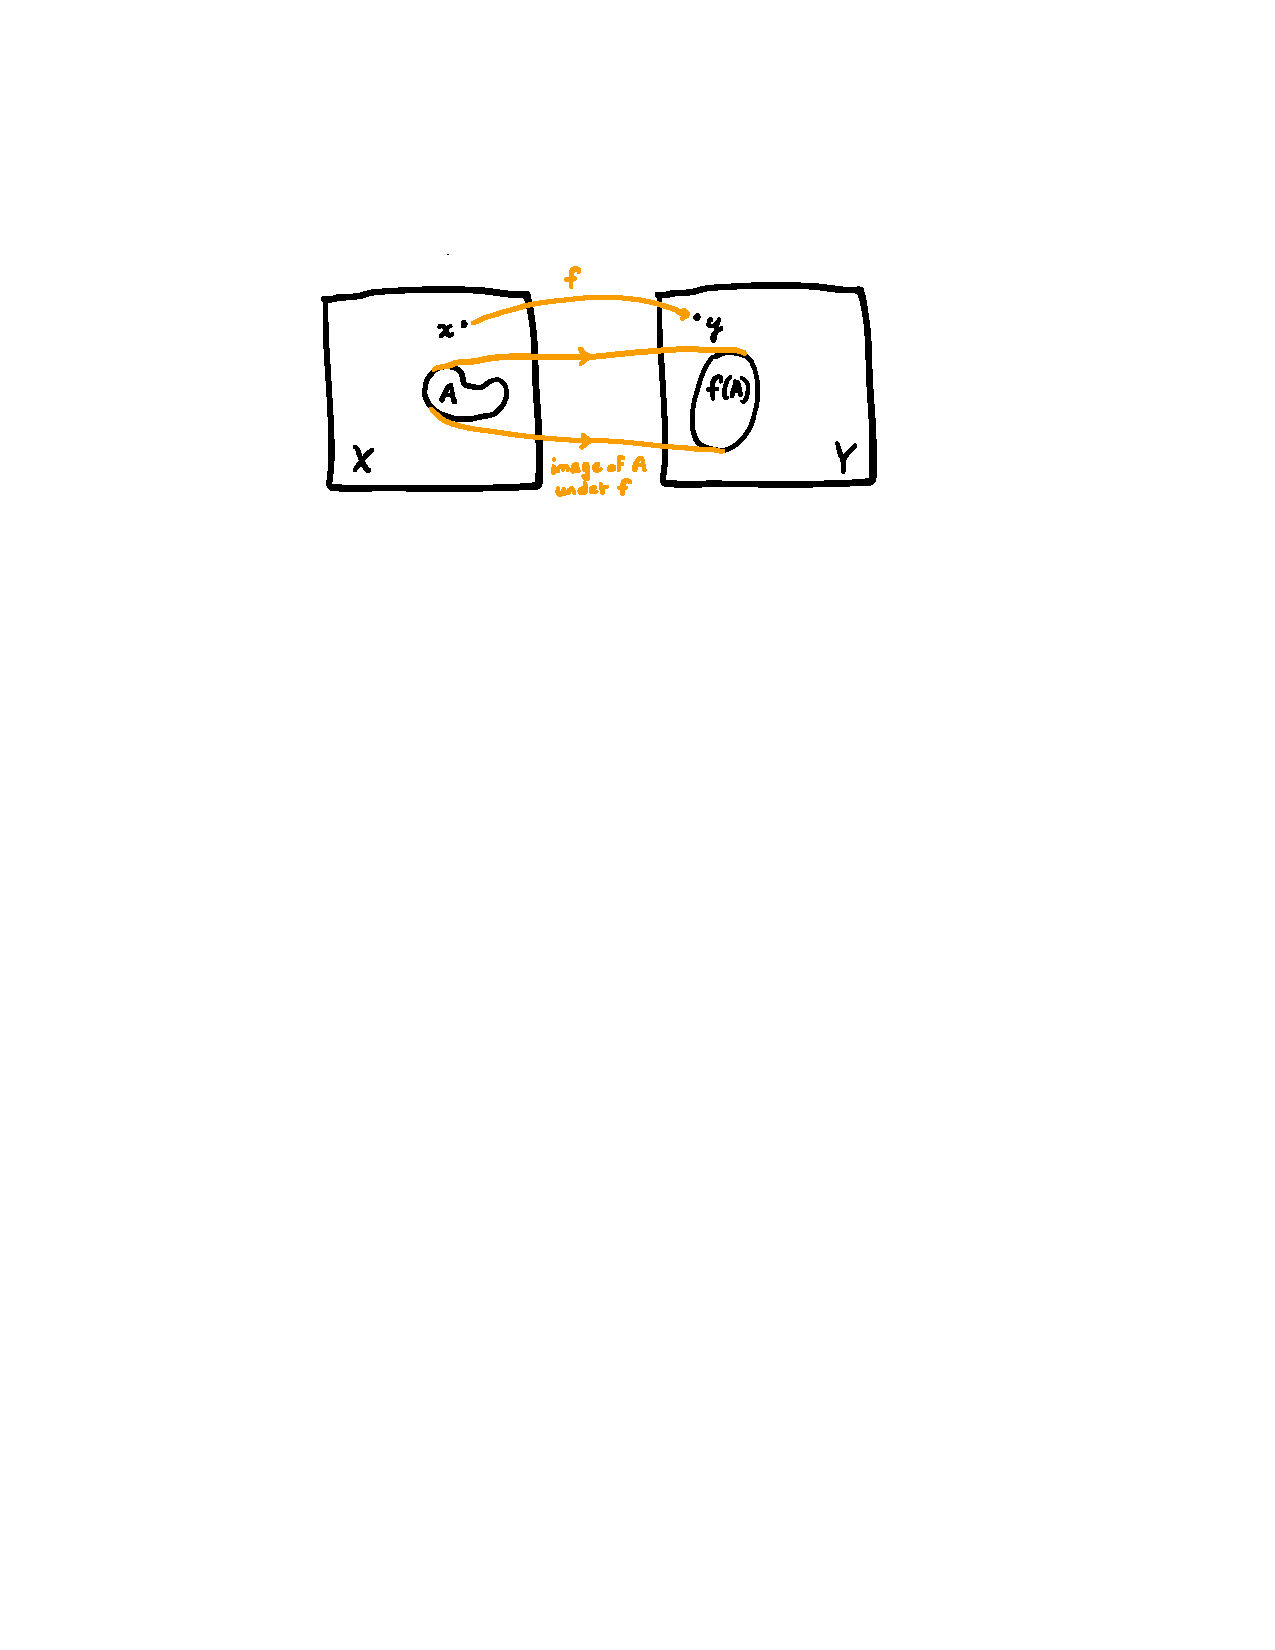
\includegraphics[width=80mm]{figures/ch1_set_image}}
\end{center}

\begin{itemize}
  \setlength\itemsep{2mm}
  \item<3-> This implies that the range of $f$ is simply $f(X)$
\end{itemize}

\note{
	\vspace{8mm}
	\begin{enumerate}[<alert@+>]
		\footnotesize
		\setlength\itemsep{3mm}
		\item Read.  
		\item Read.  Here ...
		\item Read.
	\end{enumerate}
}

\end{frame}  


\begin{frame}<1-4> \frametitle{1.5: Applying Functions to Sets (2)}

\begin{definition}<1->
The \textcolor{blue}{inverse image} or \textcolor{blue}{preimage} of a subset $C\subseteq Y$ is \vspace{-2mm}
\[ f^{-1}(C) \triangleq \{ x\in X | f(x)\in C\}. \]
\end{definition}

\begin{center}
\uncover<2->{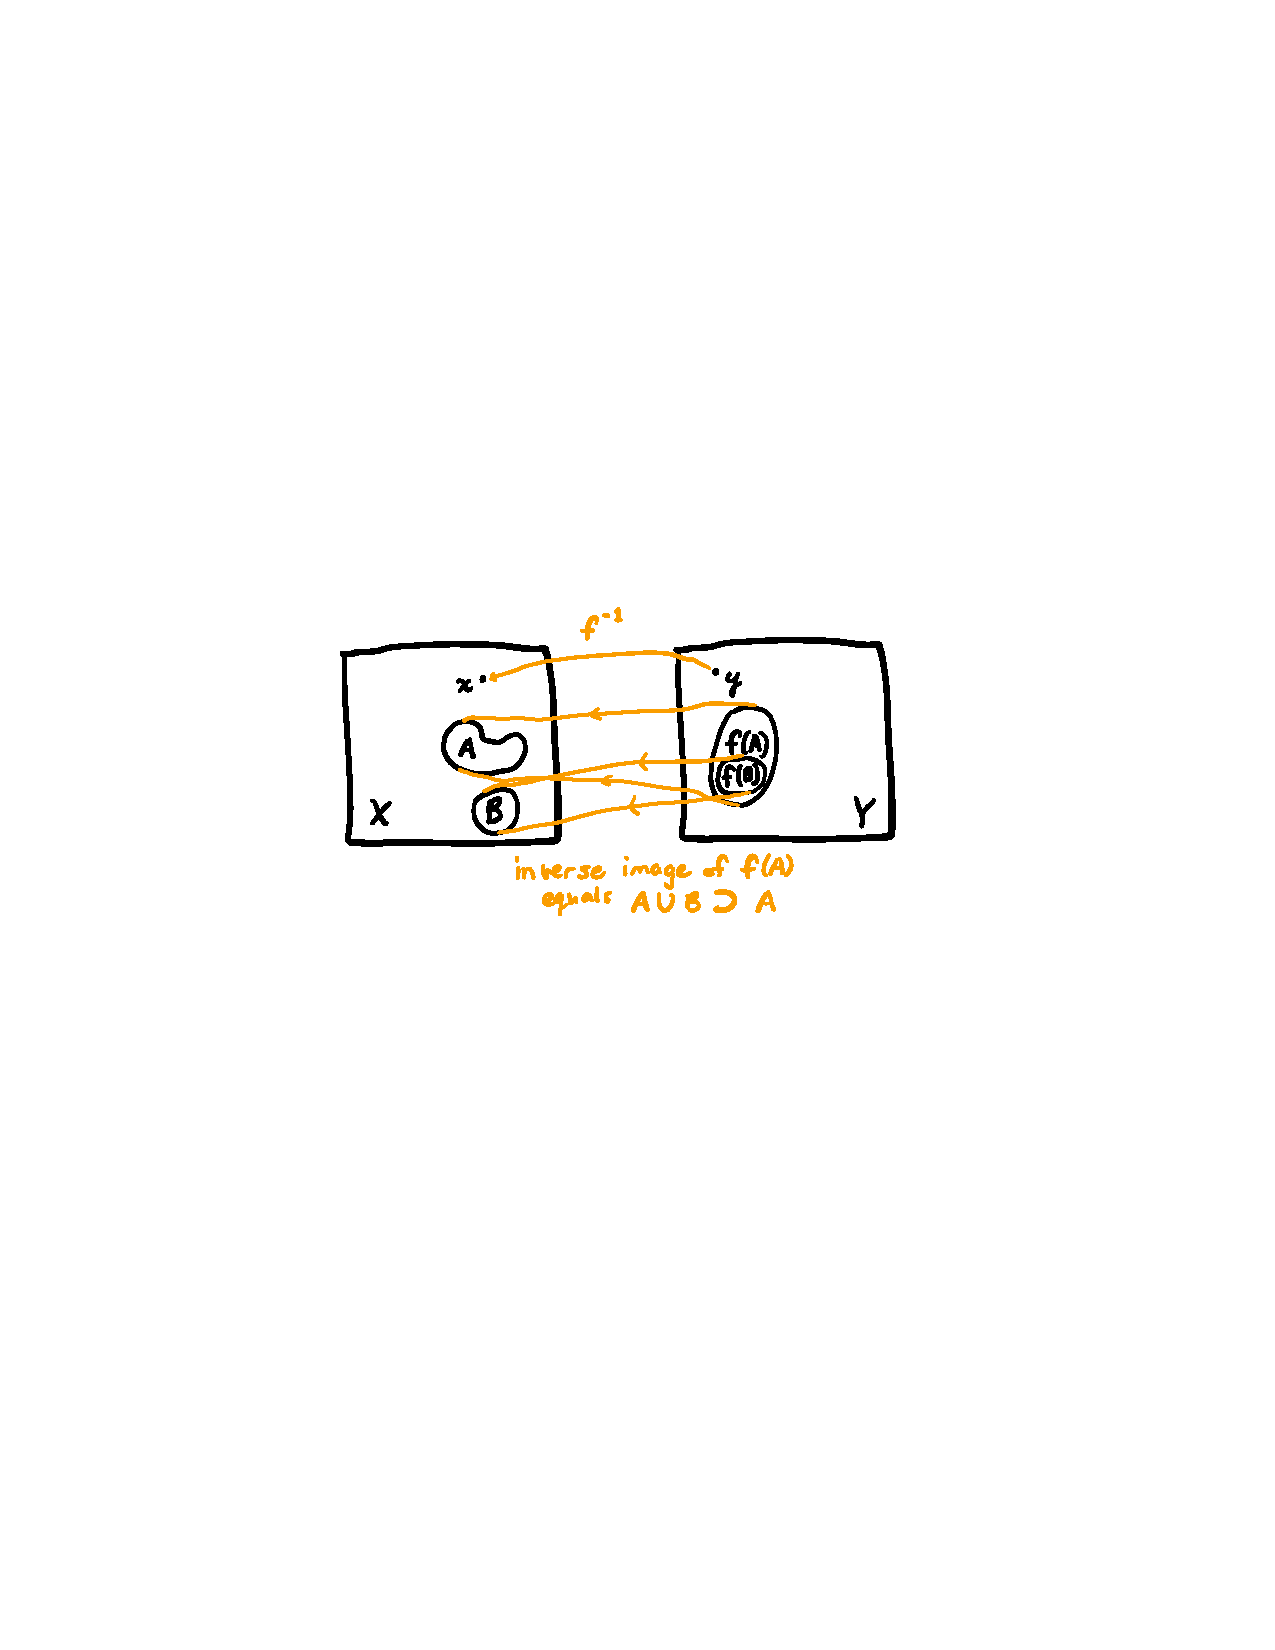
\includegraphics[width=70mm]{figures/ch1_set_inverse_image}}
\end{center}
\vspace{-2.5mm}

\begin{itemize}
  \setlength\itemsep{1.25mm}
  \item<3-> Allowing set-valued images means the \textcolor{blue}{set-valued inverse always exists}
  \item<4-> For a one-to-one $f$, the inverse image of a singleton $\{ f(x) \}$ is a singleton:$\!\!\!\!$\vspace{-0.5mm}
  \[ f^{-1}( \{f(x) \}) = \{x\} \]
  %\item<5-> In general, one can show: $f(f^{-1}(B)) \subseteq B$ and $f^{-1}(f(A)) \supseteq A$.
  %\item<6-> Ex. For $f \colon \mathbb{R} \rightarrow \mathbb{R}$ defined by $f(x)=x^2$, let $A=[1,2]$ and notice that $B = f(A) = [1,4]$.  But, $f^{-1}(B) = [-2,-1] \cup [1,2] \supseteq A$
  %\item<7-> Ex. For $f \colon \mathbb{R} \rightarrow \mathbb{R}$ defined by $f(x)=x^2+1$, let $B=[0,2]$ and notice that $A = f^{-1}(B) = [-1,1]$.  But, $f(A) = f([-1,1]) = [1,2] \subseteq B$
\end{itemize}

\note{
	\vspace{8mm}
	\begin{enumerate}[<alert@+>]
		\footnotesize
		\setlength\itemsep{3mm}
		\item Read.  
		\item Read.  Here ...
		\item Read.
	\end{enumerate}
}

\end{frame}  

\begin{frame}<1-3> \frametitle{1.5: Applying Functions to Sets (3)}

\vspace{-2mm}
\begin{center}
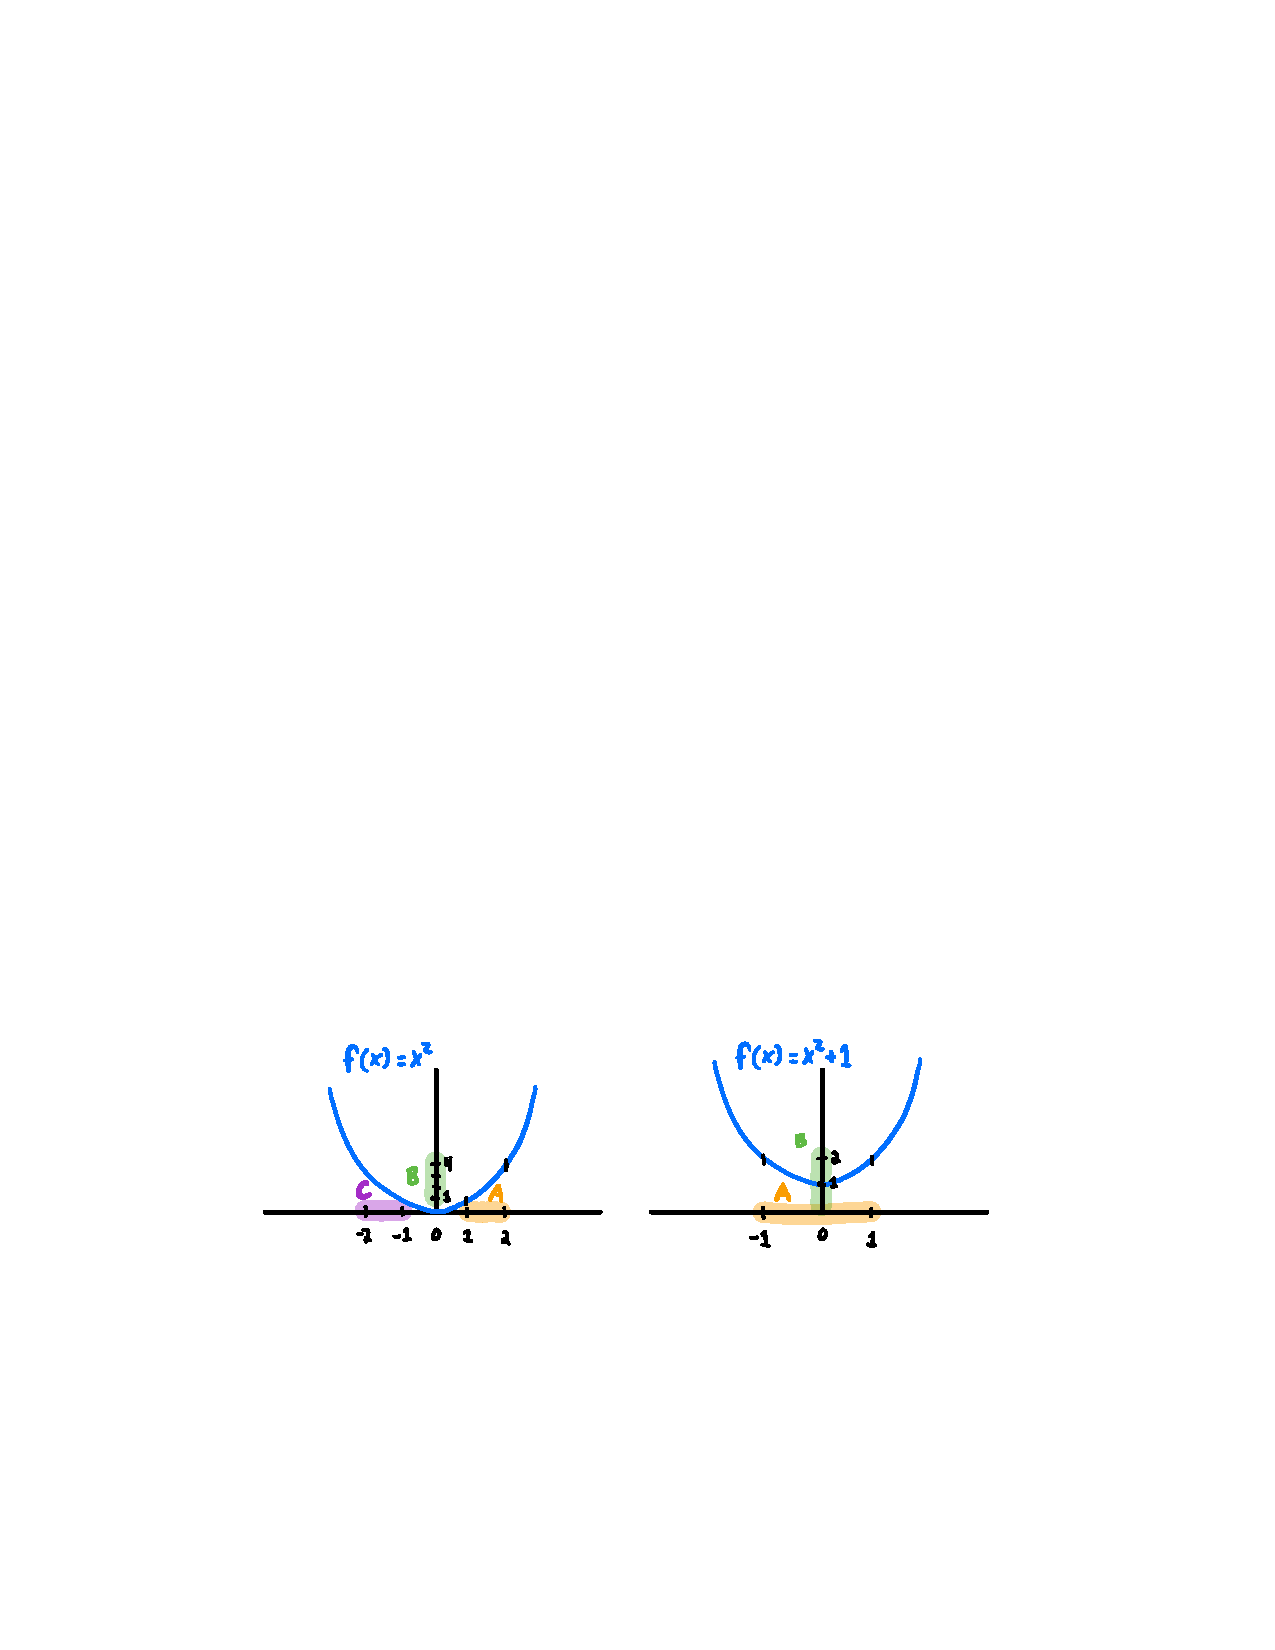
\includegraphics[width=115mm]{figures/ch1_set_image_ex}
\end{center}
\vspace{-2mm}

\begin{itemize}
    \setlength\itemsep{3mm}
    \item<1-> In general, one can show: $f^{-1}(f(A)) \supseteq A$ and $f(f^{-1}(B)) \subseteq B$
    \item<2-> Left: For $f \colon \mathbb{R} \rightarrow \mathbb{R}$ defined by $f(x)=x^2$, let $A=[1,2]$ and \\ notice that $B = f(A) = [1,4]$.  But, $f^{-1}(B) = [-2,-1] \cup [1,2] \supset A$
    \item<3-> Right: For $f \colon \mathbb{R} \rightarrow \mathbb{R}$ defined by $f(x)=x^2+1$, let $B=[0,2]$ and \\ notice that $A = f^{-1}(B) = [-1,1]$.  But, $f(A) = f([-1,1]) = [1,2] \subset B$
\end{itemize}
 

 \note{
 	\vspace{8mm}
 	\begin{enumerate}[<alert@+>]
 		\footnotesize
 		\setlength\itemsep{3mm}
 		\item Read. These expressions hold because $f$ compresses sets (i.e.,can map different inputs to the same value) while $f^{-1}$ expands sets (i.e., can map singleton to multiple values) 
 		\item Read.
 		\item Read.
 	\end{enumerate}
 }
 
 \end{frame}  
 
  
\begin{frame} \frametitle{Next Steps}

\begin{itemize}
\setlength\itemsep{5mm}
\item To continue studying after this video -- \vspace{2mm}

\begin{itemize}
 \setlength\itemsep{3mm}
 \item Try the suggested reading: Course Notes EF 1.5
 \item Or the optional reading: PAF 4.1-5.3
 \item And also looking at problems in Assignment 2
\end{itemize}
\end{itemize}

\note{
	\vspace{8mm}
	\begin{enumerate}
		\setlength\itemsep{3mm}
		\color{red}
		\item Here are some options to continue learning this material.
	\end{enumerate}
}

\end{frame}

  
\backupbegin

%\begin{frame}
%\frametitle{Backup Slides}
%\begin{itemize}
%\item Slide numbers not included in denominator!
%\end{itemize}
%\end{frame}

%\begin{frame}[allowframebreaks]
%\frametitle{References}
%\bibliographystyle{alpha}
%\footnotesize
%\bibliography{IEEEabrv,WCLabrv,WCLbib,WCLnewbib}
%\end{frame}

\backupend

\end{document}
